%!TEX root = ../../Heun_Dale_Haney_A_dynamic_approach_to_input_output_modeling.tex
%%%%%%%%%%%%%%%%%%%%% chapter.tex %%%%%%%%%%%%%%%%%%%%%%%%%%%%%%%%%
%
% sample chapter
%
% Use this file as a template for your own input.
%
%%%%%%%%%%%%%%%%%%%%%%%% Springer-Verlag %%%%%%%%%%%%%%%%%%%%%%%%%%
%\motto{Use the template \emph{chapter.tex} to style the various elements of your chapter content.}
\chapter{Energy intensity}
\label{chap:intensity} % Always give a unique label
% use \chaptermark{}
% to alter or adjust the chapter heading in the running head
\chaptermark{intensity}

In Chapter~\ref{chap:value}, we defined flows of value in an economy.
In this chapter, we merge energy and value together to estimate
the energy intensity of economic sectors.


%%%%%%%%%% Methodology %%%%%%%%%%
\section{Methodology}
%%%%%%%%%%

Energy intensity ($\varepsilon$) is the ratio 
of total energy and value outflow rates from an economic sector, 
such that for the $j^{\mathrm{th}}$ goods and services sector,

\begin{equation} \label{eq:epsilon_output_def_g_and_s}
	\varepsilon_{j} \equiv \frac{\dot{T}_{j}}{\dot{X}_{j}}.
\end{equation}

\noindent and $\varepsilon$ is in units of J/\$. 
For an energy sector, energy intensity is defined as
******** Is this next equation correct? ************

\begin{equation} \label{eq:epsilon_output_def_energy}
	\varepsilon_{j} \equiv \frac{\dot{T}_{j}}{\dot{E}_{j}} 
	= 1 + \frac{\dot{B}_{j}}{\dot{E}_{j}}.
\end{equation}

\noindent and the units of $\varepsilon$ are J/J. 
For inter-sector flows, we have

\begin{equation} \label{eq:epsilon_transfers_1}
	\varepsilon_{ij} = \frac{\dot{T}_{ij}}{\dot{X}_{ij}}.
\end{equation}

Furthermore, we note that 

\begin{equation} \label{eq:epsilon_equiv_1}
	\varepsilon_{i} = \varepsilon_{ij}
\end{equation}

\noindent for all $j$, because the energy intensity 
of sector $i$'s output is the same regardless of its destination ($j$). 
I.e., we assume that all goods produced by a sector 
are produced at the average energy intensity 
of that sector.\footnote{If this approach is unsatisfactory, 
the sector may be divided into sub-sectors 
with different energy intensities.}

We define parameter $a_{ij}$ that represents the input 
of good $i$ required to produce a unit of output from sector $j$.

\begin{equation} \label{eq:aij_def}
	a_{ij} \equiv \frac{\dot{X}_{ij}}{\dot{X}_{j}}
\end{equation}

Input-output ratios are given in mixed units, 
depending on both the purpose of each sector of the economy 
and the type of input as shown in Table~\ref{table: A_matrix_units}.

\begin{table}
\caption{Units for input-output ratios ($a$). ********** Mik: convert
this to a diagram like Figure~\ref{fig:C_mat_matrix}. **********}
\begin{center}
  \begin{tabular}{ ll | c  c | }
 			& 							& \multicolumn{2}{|c|}{Output of} \\
    		&	 						& Non-energy sector 		& Energy sector \\ \hline
\multirow{2}{*}{Inputs from}    		& Non-energy sector 	& $\frac{\text{\$}}{\text{\$}}$ 	& $\frac{\text{\$}}{\text{J}}$ \\ 
    		& Energy sector	 	& $\frac{\text{J}}{\text{\$}}$ 	& $\frac{\text{J}}{\text{J}}$ \\ \hline
  \end{tabular}
\end{center}
\label{table: A_matrix_units}
\end{table}

%%%%%%%%%% Example B %%%%%%%%%%
\section{Example B: energy intensity ($\varepsilon$)}
%%%%%%%%%%

With reference to Figures~\ref{fig:B_total_energy} and~\ref{fig:B_value}, 
the energy intensity ($\varepsilon$) 
of the energy sector (2) is given by

\begin{equation} \label{eq:single_sector_energy_intensity}
	\varepsilon_{2} = \frac{\dot{T}_{2}}{\dot{X}_{2}} = \frac{\dot{T}_{22}}{\dot{X}_{22}}.
\end{equation}

The input-output ratio ($a$) for the economic sector (2) is

\begin{equation} \label{eq:io_ratio_single_sector}
	a_{22} = \frac{\dot{X}_{22}}{\dot{X}_{2}}.
\end{equation}

\noindent Thus,

\begin{equation} \label{eq:T_dot_1_single_sector}
	\dot{T}_{2} = \varepsilon_{2}\dot{X}_{2},
\end{equation}

\noindent and

\begin{equation} \label{eq:T_dot_11_single_sector}
	\dot{T}_{22} = \varepsilon_{2}a_{22}\dot{X}_{2}.
\end{equation}

************** Need to check the following equation. ***************
Realizing that 
(a) $\frac{\mathrm{d}T_3}{\mathrm{d}t} = \frac{\mathrm{d}B_3}{\mathrm{d}t}$ 
because $\frac{\mathrm{d}E_3}{\mathrm{d}t} = 0$, 
(b) $\dot{T}_{13} = \dot{E}_{13}$ because $\dot{B}_{13} = 0$ 
due to processing of raw energy carriers occurring \emph{within} the economic sector (3), and
(c) substituting Equations~\ref{eq:T_dot_1_single_sector} 
and~\ref{eq:T_dot_11_single_sector} into Equation~\ref{eq:CV_T_3} gives

\begin{equation} \label{eq:dB1/dt_single_sector_after_substituting_eps_and_a}
	\frac{\mathrm{d}B_{2}}{\mathrm{d}t} = \varepsilon_{2}a_{22}\dot{X}_{2} + \dot{E}_{02} - \varepsilon_{2}\dot{X}_{2} - \gamma_{2}B_{2}.
\end{equation}

We can estimate the energy intensity of the economy by solving 
Equation~\ref{eq:dB1/dt_single_sector_after_substituting_eps_and_a} 
for $\varepsilon_{2}$.

\begin{equation} \label{eq:eps3_ss_IO}
	\varepsilon_{2} 
	= {(1 - a_{22})}^{-1} \dot{X}_{2}^{-1} 
	\left[\dot{E}_{02} 
	      - \left(\frac{\mathrm{d}B_{2}}{\mathrm{d}t} 
		          + \gamma_{2}B_{2}
			\right)
	\right]
\end{equation}

Equation~\ref{eq:eps3_ss_IO} is similar 
to the typical energy intensity equation 
found in the I-O literature [REFERENCE BULLARD AND OTHERS HERE. --MKH], 
except that Equation~\ref{eq:eps3_ss_IO} applies 
to a single economic sector and contains scalar 
(as opposed to matrix) terms. 
Using Example C below, we will derive 
a matrix representation of Equation~\ref{eq:eps3_ss_IO} 
that is directly comparable 
to energy intensity equations found in the I-O literature.

%%%%%%%%% Example B %%%%%%%%%%
\section{Derivation of economic sector energy intensity ($\varepsilon$) by a convergent infinite series}
%%%%%%%%%%

At this point, we will take a small aside 
to demonstrate that the single-sector economy 
of Figures~\ref{fig:direct_energy_flows} through~\ref{fig:economic_value_flows} 
can be re-drawn as shown in Figure~\ref{fig:single_sector_flows_3}.

\begin{figure}[h!]
\centering\
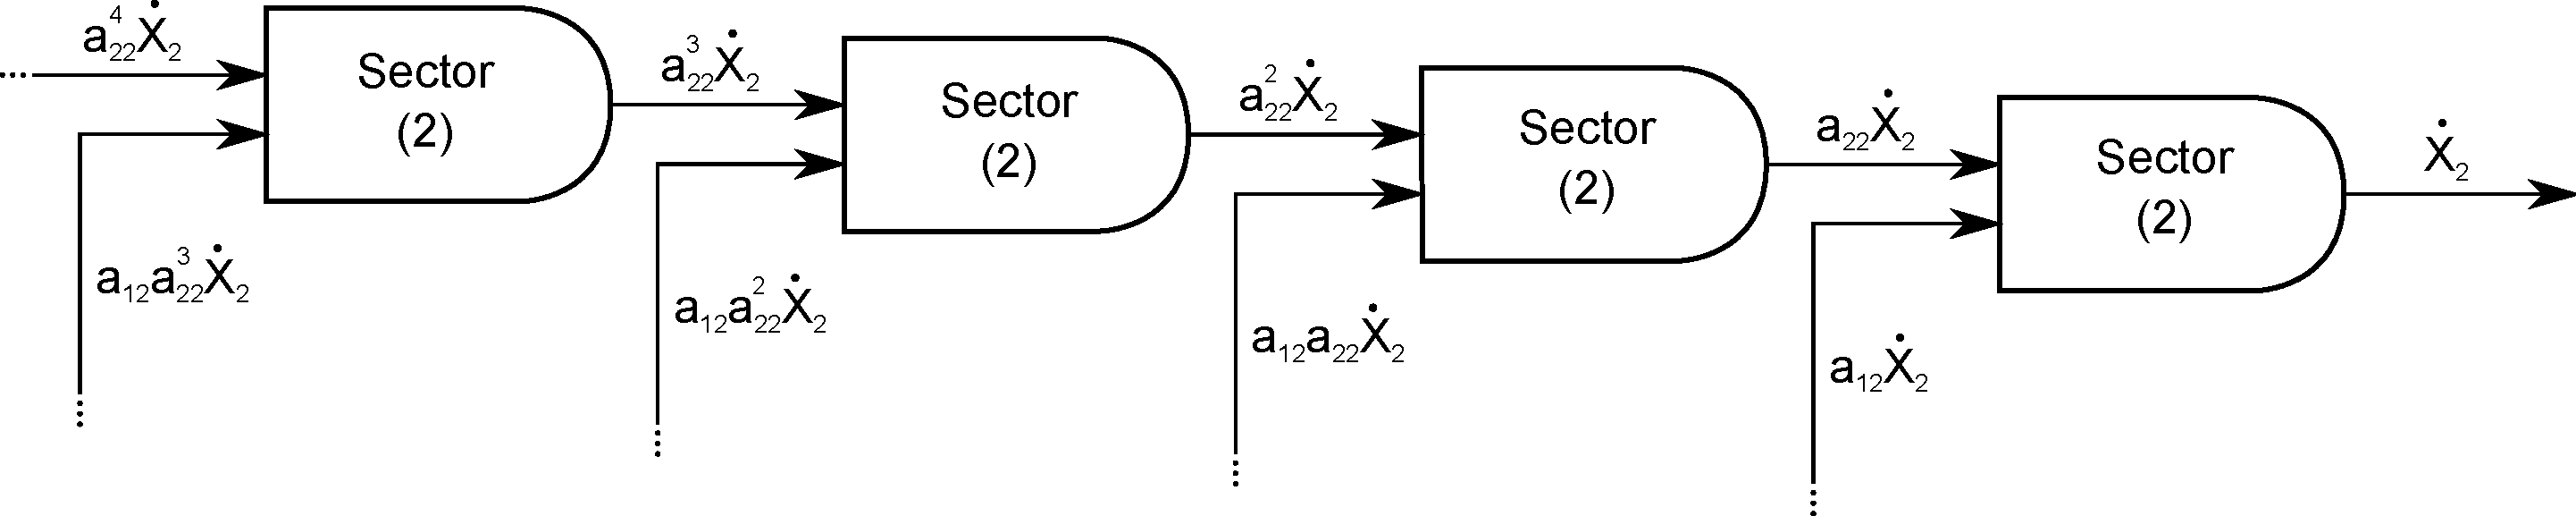
\includegraphics[width=1.0\linewidth]{Part_3/Chapter_Intensity/images/I-O_Process_Equivalence.pdf}
\caption{Process flows in a single-sector economy}{Process flows in a single-sector economy}
\label{fig:single_sector_flows_3}
\end{figure}

The economy produces output at a rate of $\dot{X}_{2}$, 
but it requires energy from the biosphere 
($\dot{E}_{02} = a_{02}\dot{X}_{2}$) to do so. 
The economy also consumes a fraction 
of its own gross output 
($\dot{X}_{22} = a_{22}\dot{X}_{2}$). 
To produce $a_{22}\dot{X}_{2}$, 
the economy requires an additional $a_{02}a_{22}\dot{X}_{2}$ 
of energy from the biosphere. 
The sum of all direct energy ($\dot{E}$) required for the economy 
to produce at a rate of $\dot{X}_{2}$ is an infinite sum.

\begin{equation} \label{eq:E_dot_demand_SS}
	\dot{E}_{demand,tot} 
	= a_{02}\dot{X}_{2} 
	+ a_{02}a_{22}\dot{X}_{2} 
	+ a_{02}a_{22}^2\dot{X}_{2} 
	+ \cdots
\end{equation}

The energy intensity of the economy ($\varepsilon_{2}$) is 

\begin{equation} \label{eq:epsilon_process_SS_intermediate}
	\varepsilon_{2} 
	= \frac{\dot{E}_{demand}}{\dot{X}_{2}} 
	= a_{02}(1 + a_{22} + a_{22}^2) + \cdots 
	= a_{02}\sum_{n=0}^{\infty}a_{22}^{n}.
\end{equation}

Realizing that $\sum_{n=0}^{\infty}a_{22}^{n} 
= \frac{1}{1-a_{22}}$ and $a_{02} 
= \frac{\dot{E}_{02}}{\dot{X}_{2}}$ gives

\begin{equation} \label{eq:epsilon_process_SS}
	\varepsilon_{2} = {(1-a_{22})}^{-1} \dot{X}^{-1} \dot{E}_{02}.
\end{equation}

Neglecting accumulation of embodied energy in the economy
$\left(\frac{\mathrm{d}B_{2}}{\mathrm{d}t}\right)$ 
and depreciation $\left(\gamma_{2}B_{2}\right)$, 
Equations~\ref{eq:eps3_ss_IO} and~\ref{eq:epsilon_process_SS} are identical 
(assuming $\frac{\mathrm{d}B_{2}}{\mathrm{d}t} =\gamma_{2} = 0$), 
indicating that the I-O approach accounts 
for the infinite recursion of energy demand by the economy.


*************** Matt ended here *************

%%%%%%%%%% Example C %%%%%%%%%%
\section{Matrix Formulation}
%%%%%%%%%%

We can use Equations~\ref{eq:epsilon_output_def} 
through~\ref{eq:epsilon_equiv_1} to rewrite 
Equations~\ref{eq:C-CV_B_1_depreciation} 
and~\ref{eq:C-CV_B_2_depreciation} as

\begin{equation} \label{eq:CV_B_3_with_eps}
	\dot{X}_{33}\varepsilon_{3} + \dot{X}_{43}\varepsilon_{4} + \dot{E}_{13} - \frac{\mathrm{d}B_{3}}{\mathrm{d}t} - \gamma_{3}B_{3} = \dot{X}_{3}\varepsilon_{3}
\end{equation}

\noindent and 

\begin{equation} \label{eq:CV_B_4_with_eps}
	\dot{X}_{34}\varepsilon_{3} + \dot{X}_{44}\varepsilon_{4} + \dot{E}_{14} - \frac{\mathrm{d}B_{4}}{\mathrm{d}t} - \gamma_{4}B_{4} = \dot{X}_{4}\varepsilon_{4}.
\end{equation}

We can rewrite Equations~\ref{eq:CV_B_3_with_eps} 
and~\ref{eq:CV_B_4_with_eps} in matrix notation with the following definitions:

\begin{equation} \label{eq:eps_vec_def}
	\vec{\varepsilon} =		\begin{Bmatrix} 	\varepsilon_{3}	\\
																\varepsilon_{4}	\\
									\end{Bmatrix},
\end{equation}

\begin{equation} \label{eq:E_vec_def}
	\vec{E} =		\begin{Bmatrix} 	\dot{E}_{13}	\\
													\dot{E}_{14}\\
						\end{Bmatrix},
\end{equation}

\begin{equation} \label{eq:dBdt_vec_def}
	\frac{\mathrm{d}\vec{B}}{\mathrm{d}t} =	\begin{Bmatrix}	\frac{\mathrm{d}B_{3}}{\mathrm{d}t}	\\
																									\frac{\mathrm{d}B_{4}}{\mathrm{d}t}\\
																		\end{Bmatrix},
\end{equation}

\begin{equation} \label{eq:B_vec_def}
	\vec{B} =			\begin{Bmatrix}	B_{3}\\
														B_{4}\\
							\end{Bmatrix},
\end{equation}

\begin{equation} \label{eq:A_matrix_def}
	\vec{A} =	\begin{bmatrix} 	a_{33} & a_{34}	\\
												a_{43} & a_{44}	\\
					\end{bmatrix},
\end{equation}

\begin{equation} \label{eq:X_t_matrix_def}
	\vec{X}_{t} =		\begin{bmatrix} 	\dot{X}_{33}		&	\dot{X}_{34}	\\
														\dot{X}_{43}		&	\dot{X}_{44}\\
							\end{bmatrix},
\end{equation}

\begin{equation} \label{eq:X_hat_matrix_def}
	\hat{\vec{X}} = \delta_{ij}\dot{X}_{j} = \begin{bmatrix} 	\dot{X}_{33}		&	0					\\
																								0					&	\dot{X}_{44}	\\
																							\end{bmatrix},
\end{equation}

\begin{equation} \label{eq:B_hat_matrix_def}
	\hat{\vec{\gamma}} = \delta_{ij}\gamma_{j},
\end{equation}

[CAN WE MAKE THIS EQUATION EXPLICIT]

\noindent and

\begin{equation}\label{eq:k_delta}
	\delta_{ij} = \begin{cases}	1 	& 	\text{if  } i = j		\\
												0	&	\text{if  } i \neq j	\\
						\end{cases},
\end{equation}

\noindent{}such that:

\begin{equation} \label{eq:matrix_leontief}
	\vec{X}_{t}^{\mathrm{T}}\vec{\varepsilon} + \vec{E} - \left(\frac{\mathrm{d}\vec{B}}{\mathrm{d}t} + \hat{\vec{\gamma}}\vec{B}\right) = \hat{\vec{X}}\vec{\varepsilon}.
\end{equation}

Additional relationships that will be helpful later include (derived in Appendix):

\begin{equation} \label{eq:Xhat_X_and_A}
	\hat{\vec{X}}^{-1}\vec{X}_{t} = \vec{A}^{\mathrm{T}},
\end{equation}

\begin{equation} \label{eq:Xdifference1}
	\vec{X}_{t}^{\mathrm{T}} - \hat{\vec{X}} = \hat{\vec{X}}(\vec{A}^{\mathrm{T}} - \vec{I}),
\end{equation}

\begin{equation} \label{eq:Xdifference2}
	\hat{\vec{X}} - \vec{X}_{t}^{\mathrm{T}} = \hat{\vec{X}}(\vec{I} - \vec{A}^{\mathrm{T}}),
\end{equation}

\noindent and

\begin{equation} \label{eq:Xdifference2_inverse}
	{\left(\hat{\vec{X}} - \vec{X}_{t}^{\mathrm{T}}\right)}^{-1} 
	= {(\vec{I} - \vec{A}^{\mathrm{T}})}^{-1}\hat{\vec{X}}^{-1}.
\end{equation}


%%%%%%%%%% Example C %%%%%%%%%%
\section{Estimating $\vec{\varepsilon}$ and $\frac{\mathrm{d}\vec{B}}{\mathrm{d}t}$}
%%%%%%%%%%

With Equation~\ref{eq:matrix_leontief}, we can solve for either 
the energy accumulation vector ($\vec{\frac{\mathrm{d}B}{\mathrm{d}t}}$) 
or the energy intensity vector ($\vec{\varepsilon}$), 
but not both. 

Solving for the accumulation vector gives

\begin{equation} \label{eq:dB_dt_leontief}
	\frac{\mathrm{d}\vec{B}}{\mathrm{d}t} = (\vec{X}_{t}^{\mathrm{T}} - \hat{\vec{X}})\vec{\varepsilon} + \vec{E} - \hat{\vec{\gamma}}\vec{B}.
\end{equation}

\noindent Finally, we can substutute Equation~\ref{eq:Xdifference1} which gives

\begin{equation} \label{eq:dB_dt_leontief_with_A}
	\frac{\mathrm{d}\vec{B}}{\mathrm{d}t} = \hat{\vec{X}} (\vec{A}^{\mathrm{T}} - \vec{I}) \vec{\varepsilon} + \vec{E} - \hat{\vec{\gamma}}\vec{B},
\end{equation}

\noindent{}which allows estimation of the embodied energy accumulation 
in economic sectors $\left(\frac{\mathrm{d}\vec{B}}{\mathrm{d}t}\right)$ 
knowing only sector outputs ($\hat{\vec{X}}$), 
sector input-output ratios ($\vec{A}$), 
sector energy intensities ($\vec{\varepsilon}$), 
energy input to the economy ($\vec{E}$), 
and sector physical depreciation rates ($\hat{\vec{\gamma}}\vec{b}$). 
In theory, the transaction matrix ($\vec{X}_{t}$) is not required 
if the input-ouput ratios ($\vec{A}$) are known, 
though in practice, knowledge of input-output ratios 
would be derived from the transaction matrix $\vec{X}_{t}$.

Solving for the energy intensity vector gives

\begin{equation} \label{eq:epsilon_leontief}
	\vec{\varepsilon} 
	= {(\hat{\vec{X}} - \vec{X}_{t}^{\mathrm{T}})}^{-1}
		\left[\vec{E} 
				- \left(\frac{\mathrm{d}\vec{B}}{\mathrm{d}t} 
				+ \hat{\vec{\gamma}}\vec{B}\right)
		\right].
\end{equation}

\noindent{}Substituting Equation~\ref{eq:Xdifference2_inverse} gives

\begin{equation} \label{eq:epsilon_leontief_with_A}
	\vec{\varepsilon} 
	= {(\vec{I} - \vec{A}^{\mathrm{T}})}^{-1}\hat{\vec{X}}^{-1}
		\left[\vec{E} 
				- \left(\frac{\mathrm{d}\vec{B}}{\mathrm{d}t} 
				+ \hat{\vec{\gamma}}\vec{B}\right)
		\right],
\end{equation}

\noindent{}which allows estimation of the energy intensity of economic sectors ($\vec{\varepsilon}$) knowing only sector input-output ratios ($\vec{A}$), sector outputs ($\hat{\vec{X}}$), energy input to the economy ($\vec{E}$), sector embodied energy accumulation rates $\left(\frac{\mathrm{d}\vec{B}}{\mathrm{d}t}\right)$, and sector physical depreciation rates ($\hat{\vec{\gamma}}\vec{B}$).

Comparison of Equations~\ref{eq:eps1_ss_IO} and~\ref{eq:epsilon_leontief_with_A} shows the similarities between the single-sector algebraic formulation and the multi-sector matrix formulation of the I-O analysis method. This newly developed multi-sector matrix formulation can be extended to any desired level of economic and energy sector disaggregation as shown by Bullard (1975, 1978) and others.

************************** MATT ENDED HERE *************************


%%%%%%%%%% Intensity: Auto industry example %%%%%%%%%%
\section{Energy intensity of the auto industry}
\label{sec:intensity_auto}
%%%%%%%%%%

%%%%%%%%%% Intensity: Summary %%%%%%%%%%
\section{Summary}
\label{sec:intensity_summary}
%%%%%%%%%%

\abstract*{[NEED TO ADD ABSTRACT HERE]}

%% \abstract{Each chapter should be preceded by an abstract (10--15 lines long) that summarizes the content. The abstract will appear \textit{online} at \url{www.SpringerLink.com} and be available with unrestricted access. This allows unregistered users to read the abstract as a teaser for the complete chapter. As a general rule the abstracts will not appear in the printed version of your book unless it is the style of your particular book or that of the series to which your book belongs.\newline\indent
%% Please use the 'starred' version of the new Springer \texttt{abstract} command for typesetting the text of the online abstracts (cf. source file of this chapter template \texttt{abstract}) and include them with the source files of your manuscript. Use the plain \texttt{abstract} command if the abstract is also to appear in the printed version of the book.}

%% Use the template \emph{chapter.tex} together with the Springer document class SVMono (monograph-type books) or SVMult (edited books) to style the various elements of your chapter content in the Springer layout.




\bibliographystyle{unsrt}
\bibliography{../../EROI_review_v2}


% Always give a unique label
% and use \ref{<label>} for cross-references
% and \cite{<label>} for bibliographic references
% use \sectionmark{}
% to alter or adjust the section heading in the running head
%% Instead of simply listing headings of different levels we recommend to let every heading be followed by at least a short passage of text. Furtheron please use the \LaTeX\ automatism for all your cross-references and citations.

%% Please note that the first line of text that follows a heading is not indented, whereas the first lines of all sequent paragraphs are.

%% Use the standard \verb|equation| environment to typeset your equations, e.g.
%
%% \begin{equation}
%% a \times b = c\;,
%% \end{equation}
%
%% however, for multiline equations we recommend to use the \verb|eqnarray|
%% environment\footnote{In physics texts please activate the class option \texttt{vecphys} to depict your vectors in \textbf{\itshape boldface-italic} type - as is customary for a wide range of physical jects.}.
%% \begin{eqnarray}
%% a \times b = c \nonumber\\
%% \vec{a} \cdot \vec{b}=\vec{c}
%% \label{eq:01}
%% \end{eqnarray}

%% \section{section Heading}
%% \label{sec:2}
%% Instead of simply listing headings of different levels we recommend to let every heading be followed by at least a short passage of text. Furtheron please use the \LaTeX\ automatism for all your cross-references\index{cross-references} and citations\index{citations} as has already been described in Sect.~\ref{sec:2}.

%% \begin{quotation}
%% Please do not use quotation marks when quoting texts! Simply use the \verb|quotation| environment -- it will automatically render Springer's preferred layout.
%% \end{quotation}


%% \section{section Heading}
%% Instead of simply listing headings of different levels we recommend to let every heading be followed by at least a short passage of text. Furtheron please use the \LaTeX\ automatism for all your cross-references and citations as has already been described in Sect.~\ref{sec:2}, see also Fig.~\ref{fig:1}\footnote{If you copy text passages, figures, or tables from other works, you must obtain \textit{permission} from the copyright holder (usually the original publisher). Please enclose the signed permission with the manucript. The sources\index{permission to print} must be acknowledged either in the captions, as footnotes or in a separate section of the book.}

%% Please note that the first line of text that follows a heading is not indented, whereas the first lines of all sequent paragraphs are.

% For figures use
%
%% \begin{figure}[b]
%% \sidecaption
% Use the relevant command for your figure-insertion program
% to insert the figure file.
% For example, with the option graphics use
%% \includegraphics[scale=.65]{figure}
%
% If not, use
%\picplace{5cm}{2cm} % Give the correct figure height and width in cm
%
%% \caption{If the width of the figure is less than 7.8 cm use the \texttt{sidecapion} command to flush the caption on the left side of the page. If the figure is positioned at the top of the page, align the sidecaption with the top of the figure -- to achieve this you simply need to use the optional argument \texttt{[t]} with the \texttt{sidecaption} command}
%% \label{fig:1}       % Give a unique label
%% \end{figure}


%% \paragraph{Paragraph Heading} %
%% Instead of simply listing headings of different levels we recommend to let every heading be followed by at least a short passage of text. Furtheron please use the \LaTeX\ automatism for all your cross-references and citations as has already been described in Sect.~\ref{sec:2}.

%% Please note that the first line of text that follows a heading is not indented, whereas the first lines of all sequent paragraphs are.

%% For typesetting numbered lists we recommend to use the \verb|enumerate| environment -- it will automatically render Springer's preferred layout.

%% \begin{enumerate}
%% \item{Livelihood and survival mobility are oftentimes coutcomes of uneven socioeconomic development.}
%% \begin{enumerate}
%% \item{Livelihood and survival mobility are oftentimes coutcomes of uneven socioeconomic development.}
%% \item{Livelihood and survival mobility are oftentimes coutcomes of uneven socioeconomic development.}
%% \end{enumerate}
%% \item{Livelihood and survival mobility are oftentimes coutcomes of uneven socioeconomic development.}
%% \end{enumerate}


%% \paragraph{paragraph Heading} In order to avoid simply listing headings of different levels we recommend to let every heading be followed by at least a short passage of text. Use the \LaTeX\ automatism for all your cross-references and citations as has already been described in Sect.~\ref{sec:2}, see also Fig.~\ref{fig:2}.

%% Please note that the first line of text that follows a heading is not indented, whereas the first lines of all sequent paragraphs are.

%% For unnumbered list we recommend to use the \verb|itemize| environment -- it will automatically render Springer's preferred layout.

%% \begin{itemize}
%% \item{Livelihood and survival mobility are oftentimes coutcomes of uneven socioeconomic development, cf. Table~\ref{tab:1}.}
%% \begin{itemize}
%% \item{Livelihood and survival mobility are oftentimes coutcomes of uneven socioeconomic development.}
%% \item{Livelihood and survival mobility are oftentimes coutcomes of uneven socioeconomic development.}
%% \end{itemize}
%% \item{Livelihood and survival mobility are oftentimes coutcomes of uneven socioeconomic development.}
%% \end{itemize}

%% \begin{figure}[t]
%% \sidecaption[t]
% Use the relevant command for your figure-insertion program
% to insert the figure file.
% For example, with the option graphics use
%% \includegraphics[scale=.65]{figure}
%
% If not, use
%\picplace{5cm}{2cm} % Give the correct figure height and width in cm
%
%% \caption{Please write your figure caption here}
%% \label{fig:2}       % Give a unique label
%% \end{figure}

%% \runinhead{Run-in Heading Boldface Version} Use the \LaTeX\ automatism for all your cross-references and citations as has already been described in Sect.~\ref{sec:2}.

%% \runinhead{Run-in Heading Italic Version} Use the \LaTeX\ automatism for all your cross-refer\-ences and citations as has already been described in Sect.~\ref{sec:2}\index{paragraph}.
% Use the \index{} command to code your index words
%
% For tables use
%
%% \begin{table}
%% \caption{Please write your table caption here}
%% \label{tab:1}       % Give a unique label
%
% For LaTeX tables use
%
%% \begin{tabular}{p{2cm}p{2.4cm}p{2cm}p{4.9cm}}
%% \hline\noalign{\smallskip}
%% Classes & class & Length & Action Mechanism  \\
%% \noalign{\smallskip}\svhline\noalign{\smallskip}
%% Translation & mRNA$^a$  & 22 (19--25) & Translation repression, mRNA cleavage\\
%% Translation & mRNA cleavage & 21 & mRNA cleavage\\
%% Translation & mRNA  & 21--22 & mRNA cleavage\\
%%Translation & mRNA  & 24--26 & Histone and DNA Modification\\
%%\noalign{\smallskip}\hline\noalign{\smallskip}
%%\end{tabular}
%%$^a$ Table foot note (with superscript)
%%\end{table}
%
%% \section{Section Heading}
%%\label{sec:3}
% Always give a unique label
% and use \ref{<label>} for cross-references
% and \cite{<label>} for bibliographic references
% use \sectionmark{}
% to alter or adjust the section heading in the running head
%% Instead of simply listing headings of different levels we recommend to let every heading be followed by at least a short passage of text. Furtheron please use the \LaTeX\ automatism for all your cross-references and citations as has already been described in Sect.~\ref{sec:2}.

%% Please note that the first line of text that follows a heading is not indented, whereas the first lines of all sequent paragraphs are.

%%If you want to list definitions or the like we recommend to use the Springer-enhanced \verb|description| environment -- it will automatically render Springer's preferred layout.

%%\begin{description}[Type 1]
%%\item[Type 1]{That addresses central themes pertainng to migration, health, and disease. In Sect.~\ref{sec:1}, Wilson discusses the role of human migration in infectious disease distributions and patterns.}
%%\item[Type 2]{That addresses central themes pertainng to migration, health, and disease. In Sect.~\ref{sec:2}, Wilson discusses the role of human migration in infectious disease distributions and patterns.}
%%\end{description}

%%\section{section Heading} %
%% In order to avoid simply listing headings of different levels we recommend to let every heading be followed by at least a short passage of text. Use the \LaTeX\ automatism for all your cross-references and citations citations as has already been described in Sect.~\ref{sec:2}.

%% Please note that the first line of text that follows a heading is not indented, whereas the first lines of all sequent paragraphs are.

%% \begin{svgraybox}
%% If you want to emphasize complete paragraphs of texts we recommend to use the newly defined Springer class option \verb|graybox| and the newly defined environment \verb|svgraybox|. This will produce a 15 percent screened box 'behind' your text.

%% If you want to emphasize complete paragraphs of texts we recommend to use the newly defined Springer class option and environment \verb|svgraybox|. This will produce a 15 percent screened box 'behind' your text.
%% \end{svgraybox}


%% \section{section Heading}
%%Instead of simply listing headings of different levels we recommend to let every heading be followed by at least a short passage of text. Furtheron please use the \LaTeX\ automatism for all your cross-references and citations as has already been described in Sect.~\ref{sec:2}.

%% Please note that the first line of text that follows a heading is not indented, whereas the first lines of all sequent paragraphs are.

%% \begin{theorem}
%% Theorem text goes here.
%% \end{theorem}
%
% or
%
%% \begin{definition}
%% Definition text goes here.
%% \end{definition}

%% \begin{proof}
%\smartqed
%% Proof text goes here.
%% \qed
%% \end{proof}

%%\paragraph{Paragraph Heading} %
%% Instead of simply listing headings of different levels we recommend to let every heading be followed by at least a short passage of text. Furtheron please use the \LaTeX\ automatism for all your cross-references and citations as has already been described in Sect.~\ref{sec:2}.

%% Note that the first line of text that follows a heading is not indented, whereas the first lines of all subsequent paragraphs are.
%
% For built-in environments use
%
%%\begin{theorem}
%%Theorem text goes here.
%%\end{theorem}
%
%%\begin{definition}
%%Definition text goes here.
%%\end{definition}
%
%%\begin{proof}
%%\smartqed
%% Proof text goes here.
%%\qed
%%\end{proof}
%
%% \begin{acknowledgement}
%% If you want to include acknowledgments of assistance and the like at the end of an individual chapter please use the \verb|acknowledgement| environment -- it will automatically render Springer's preferred layout.
%% \end{acknowledgement}
%
%% \section*{Appendix}
%% \addcontentsline{toc}{section}{Appendix}
%
%% When placed at the end of a chapter or contribution (as opposed to at the end of the book), the numbering of tables, figures, and equations in the appendix section continues on from that in the main text. Hence please \textit{do not} use the \verb|appendix| command when writing an appendix at the end of your chapter or contribution. If there is only one the appendix is designated ``Appendix'', or ``Appendix 1'', or ``Appendix 2'', etc. if there is more than one.

%% \begin{equation}
%% a \times b = c
%% \end{equation}
% Problems or Exercises should be sorted chapterwise
%% \section*{Problems}
%% \addcontentsline{toc}{section}{Problems}
%
% Use the following environment.
% Don't forget to label each problem;
% the label is needed for the solutions' environment
%% \begin{prob}
%% \label{prob1}
%% A given problem or Excercise is described here. The
%% problem is described here. The problem is described here.
%% \end{prob}

%% \begin{prob}
%% \label{prob2}
%% \textbf{Problem Heading}\\
%% (a) The first part of the problem is described here.\\
%% (b) The second part of the problem is described here.
%% \end{prob}


